\documentclass[a4paper]{article} 
\addtolength{\hoffset}{-2.25cm}
\addtolength{\textwidth}{4.5cm}
\addtolength{\voffset}{-3.25cm}
\addtolength{\textheight}{5cm}
\setlength{\parskip}{0pt}
\setlength{\parindent}{0in}

%----------------------------------------------------------------------------------------
%	PACKAGES AND OTHER DOCUMENT CONFIGURATIONS
%----------------------------------------------------------------------------------------

\usepackage{blindtext} % Package to generate dummy text
\usepackage{charter} % Use the Charter font
\usepackage[utf8]{inputenc} % Use UTF-8 encoding
\usepackage{microtype} % Slightly tweak font spacing for aesthetics
\usepackage[english, ngerman]{babel} % Language hyphenation and typographical rules
\usepackage{amsthm, amsmath, amssymb} % Mathematical typesetting
\usepackage{float} % Improved interface for floating objects
\usepackage[final, colorlinks = true, 
            linkcolor = black, 
            citecolor = black]{hyperref} % For hyperlinks in the PDF
\usepackage{graphicx, multicol} % Enhanced support for graphics
\usepackage{xcolor} % Driver-independent color extensions
\usepackage{marvosym, wasysym} % More symbols
\usepackage{rotating} % Rotation tools
\usepackage{censor} % Facilities for controlling restricted text
\usepackage{listings, style/lstlisting} % Environment for non-formatted code, !uses style file!
\usepackage{pseudocode} % Environment for specifying algorithms in a natural way
\usepackage{style/avm} % Environment for f-structures, !uses style file!
\usepackage{booktabs} % Enhances quality of tables
\usepackage{tikz-qtree} % Easy tree drawing tool
\tikzset{every tree node/.style={align=center,anchor=north},
         level distance=2cm} % Configuration for q-trees
\usepackage{style/btree} % Configuration for b-trees and b+-trees, !uses style file!
\usepackage[backend=biber,style=numeric,
            sorting=nyt]{biblatex} % Complete reimplementation of bibliographic facilities
\addbibresource{ecl.bib}
\usepackage{csquotes} % Context sensitive quotation facilities
\usepackage[yyyymmdd]{datetime} % Uses YEAR-MONTH-DAY format for dates
\usepackage{comment}
\renewcommand{\dateseparator}{-} % Sets dateseparator to '-'
\usepackage{fancyhdr} % Headers and footers
\pagestyle{fancy} % All pages have headers and footers
\fancyhead{}\renewcommand{\headrulewidth}{0pt} % Blank out the default header
\fancyfoot[L]{ECSE 683 - Assignment 2} % Custom footer text
\fancyfoot[C]{Nithilasaravanan Kuppan} % Custom footer text
\fancyfoot[R]{\thepage} % Custom footer text
\newcommand{\note}[1]{\marginpar{\scriptsize \textcolor{red}{#1}}} % Enables comments in red on margin

%----------------------------------------------------------------------------------------

\begin{document}

%-------------------------------
%	TITLE SECTION
%-------------------------------

\fancyhead[C]{}
\hrule \medskip % Upper rule
\begin{minipage}{0.295\textwidth} 
\raggedright
\footnotesize
NITHILASARAVANAN KUPPAN \hfill\\   
260905444\hfill\\
nithilasaravana.kuppan@mail.mcgill.ca
\end{minipage}
\begin{minipage}{0.4\textwidth} 
\centering 
\large 
ECSE 683: Assignment 2\\ 
\normalsize 
Writing Characters\\ 
\end{minipage}
\begin{minipage}{0.295\textwidth} 
\raggedleft
{\text November 15, 2020}\hfill\\
\end{minipage}
\medskip\hrule 
\bigskip

%-------------------------------
%	CONTENTS
%-------------------------------

\section{INTRODUCTION}
The objective of this assignment was to generate a set of trajectories using imitation learning. The task was to reproduce at least 3 characters while staying within the robot's practical limits. From a multitude of possible solutions, this document will illustrate one such solution that utilizes a powerful regression technique to successfully complete the aforementioned task.\\

For this solution, {\it PyBullet} was used which is a Python module dedicated towards robotic simulation; {\it Kuka IIWA} was the chosen robot for this process. The detailed procedure and algorithms will be discussed in the later sections but learning of the parameters was done via \textbf{Imitation Learning}, specifically using a regression algorithm called{ \it Random Forests}. Inverse Kinematics control was applied to the end effector to effectively track the path generated by the algorithm. \\

Since {\it Kuka IIWA} has 7 joints, the configuration space can be represented as \textbf{$\mathbb{R}^7$} and the Degree of Freedom as \textbf{7}. The task space is produced by the end effector of the Kuka robot which is \textbf{$\mathbb{R}^3$} with \textbf{3} Degrees of Freedom.\\

The presented solution uses an Inverse Kinematics control which takes in the predicted velocities of the end effector as the input and outputs all the corresponding joint velocities and then these are fed into a {\it setJointMotorControl2} function {\it (leveraging velocity control)} that converts it into proper torques that move the different links of the arm according to the velocities. \\

Since the script does take position as an input and the model outputs predicted velocities, it would be logical to conclude that the \textbf{state} is the \textbf{position} of the end effector and \textbf{action} is the \textbf{output velocity} i.e., the {\it end effector velocity}, which is in turn used to calculate the joint velocities using pseudo inverse of the Jacobian.\\

The following section provides an incisive look into the method used to solve this problem.
\bigskip


\section{METHOD}
Essentially, to solve this problem, the two following steps were performed
\begin{enumerate}
    \item Finding the velocity required to track the path of a character
    \item Using this velocity effectively on the robot
\end{enumerate}

\subsection{\it \textbf{Imitation Learning as a Regression Problem}}
The first step was to collect or obtain trajectory data for all these characters, specifically all the English alphabets. Such a set of characters were borrowed from the source codes of the python library {\it PbDlib}, which is a package for robot programming by demonstration {\it (learning from demonstration)}. This data has been stored in the repository under {\it data/2Dletters} - this folder has all the {\it .mat} files containing trajectory information {\it (position and velocity)} required for tracking alphabets.\\

After leveraging {\it scipy} to convert {\it .mat} files into python readable files {\it (nested lists of positions and their corresponding velocities)} the data was split into train and test. From $n$ sets of trajectories, $n - 1$ were used for training and one was used to test / predict the velocities. The presented solution looks at this problem like a regression task - the {\it position} columns can be taken as \textbf{features} and their corresponding velocities as \textbf{target variables}.\\

This regression task was solved using {\it Random Forests}. {\it Random forest} is a supervised learning algorithm which uses ensemble learning method {\it (technique that combines the predictions from multiple machine learning algorithms together to make more accurate predictions)} for classification and regression. The algorithm constructs multiple decision trees using the training data and churning out the mean prediction of those trees. Python's {\it scikit-learn} library provides a set of easy to use functions to code this algorithm and this solution leverages the same. After a considerable amount of experimenting with the model, a set of hyperparameters were decided upon and finalized for this script {\it (exact values of the parameters are given in the experiments section)}.


\subsection{\it \textbf{Predicted Velocity based Robot Tracking}}

Before using this predicted velocity as an input for the robot, slight modifications need to be made to make it more conducive for a practical simulation environment - 
\begin{enumerate}
    \item The trajectory data that was used for modelling was collected on a flat 2D surface, from a tablet. And hence, it is important to scale those velocities for them to work efficiently in a 3D environment. Therefore, it is of utmost importance to scale the velocity to successfully cater writing {\it multiple} characters while not violating the physical limits of the robot - This was achieved simply by scaling the output by a constant
    \item Writing characters is a 2D task, but since this solution simulates a 3D robot arm in Python {\it (specifically, Kuka IIWA robot)} a third dimension must be added {\it (with a value of 0 since the robot only needs to move in 2 dimensions)}
\end{enumerate}
Once these velocities {\it (which are technically the end effector velocities)} were obtained, the corresponding joint velocities were calculated using pseudo inverse of their respective Jacobians and were then supplied to the robot. The base code for robot simulation was taken from the {\it previous assignment submission}, which in turn referred to Prof. Hsiu-Chin Lin's {\it Course Example Repo}.

\bigskip

\section{EXPERIMENTS}
\subsection{Model Parameters}
After multiple rounds of evaluating different types of non linear regression techniques, {\it Random Forests} was finalized with the following parameters -
\\
\begin{center}
 \begin{tabular}{| c | c | c |} 
 \hline
 \textbf{Parameter Name} & \textbf{Short Explanation} & \textbf{Parameter Value} \\ [0.5ex] 
 \hline
 n\_estimators & {\it \# trees} & 1000  \\ 
 \hline
 criterion & {\it func. to measure split quality} & {\it mse} \\
 \hline
 oob\_score & {\it toggle out-of-bag sampling} & {\it True} \\
[0.5ex] 
 \hline
\end{tabular}
\end{center}
\\
\subsection{Character Selection}
As mentioned in the last section, the velocities were scaled down by a factor of 40. This was done to bring the velocities to the robot's limit {\it (a function was also created to check whether the velocities are in range for every control cycle)} and to enable writing multiple characters, all while being in the range of the robot.\\

While testing out trajectory data for different characters, it was seen that characters that can be written in a single stroke {\it(or characters that only have one possible direction to proceed in, at every point)} work flawlessly while complex characters that cannot be written in one stroke perform bad. Two metrics were calculated on the trajectory data for all the characters that were tested - {\it mean squared error} \& {\it R2 score}. An {\it R2 score} of 1 would mean that the predicted velocity perfectly overlays the test velocity and a negative score would mean that the predicted values are useless.\\

It was seen that single stroke characters like C, D, G, L, N, O, etc all have a good R2 score of 0.75 or above. The non linear regression algorithm successfully predicted the velocities corresponding to the input positions, engendering near perfect paths for the robot to follow. Even some complex characters like M, A, W had a decent score of 0.5 or above and the robot was able to {\it imperfectly} reciprocate the intended shape. However, multi stroke characters like H, X, Y, K all had very less scores, possibly even negative scores and the robot could not follow the output velocities to track these characters. \\

Following much testing and experimenting, the letters in the word \textbf{'GROWL'} was decided to be target letters for the robot to {\it write}. The following images are screenshots of the metrics generated from the model {\it (these values were captured from STDOUT console)}.\\

\begin{center}
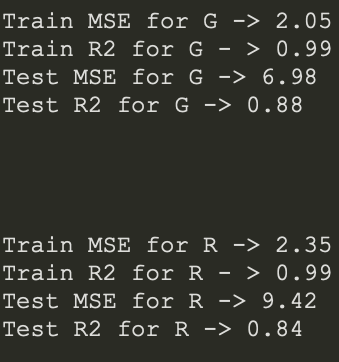
\includegraphics[scale=0.75]{images/3_1.png}  
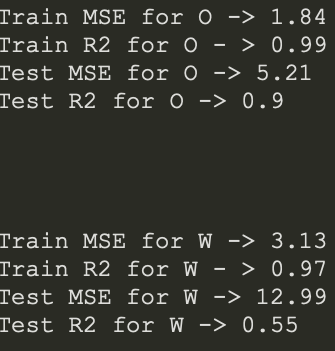
\includegraphics[scale=0.75]{images/3_2.png}  
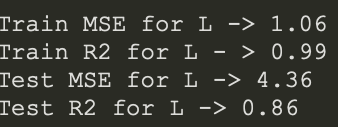
\includegraphics[scale=0.75]{images/3_3.png}
\end{center}

\subsection{Velocity Limit Checker}

A function called {\it velocityInRange()} was used to check whether the velocities being fed every control cycle are within the range for the robot. Since the predicted end effector velocities are assured to be in range {\it (because of scaling them down earlier)}, the joint velocities calculated by inverse kinematics were fed into this function. A dot (.) was output to STDOUT if it passed the limit check {\it (the limit in the urdf file was $\pm 10$ but to be even safer, the function uses $\pm 8$) } and if the check fails, an error message would be printed to STDOUT and the script would terminate. The following is the screenshot of the STDOUT console that shows this function in action\\

\begin{center}
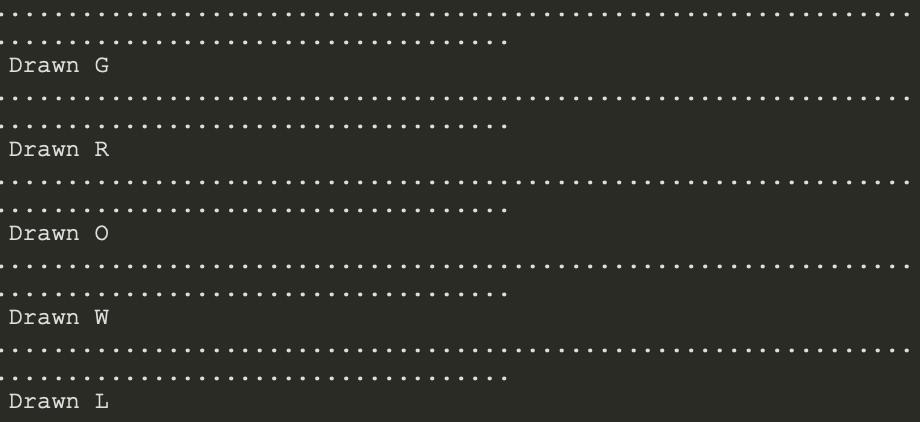
\includegraphics[scale=0.6]{images/4.png}
\end{center}

\subsection{Character to Character Movement}
Since the selected task involves writing the word \textbf{'GROWL'}, the arm needs to be initially positioned in a way that the whole word fits into the range of the robot - for this reason, the starting point was moved a bit farther left to 
[-0.3, 0.7, 0.3]. Additionally, it is important to allow some gap between each of these letters - this was achieved by setting an appropriate velocity and feeding it in between the block of code writing each of the designated letters. One such instance has been demonstrated below - \\
\begin{center}
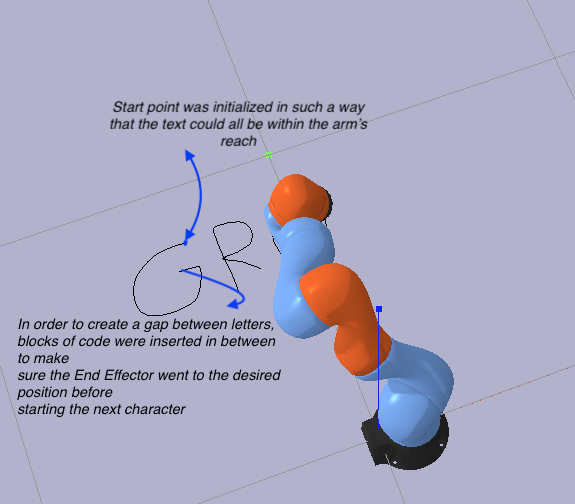
\includegraphics[scale=0.9]{images/1.png} \\
\end{center}

A screenshot of the final finished simulation has been pasted below. Please refer to {\it Demonstration\_Assign2.mp4} in the repository for the complete video. It can be clearly seen that the letter 'W' is not perfect {\it (has an R2 score of 0.55)} but its still legible enough to be called a 'W'. \\
\begin{center}
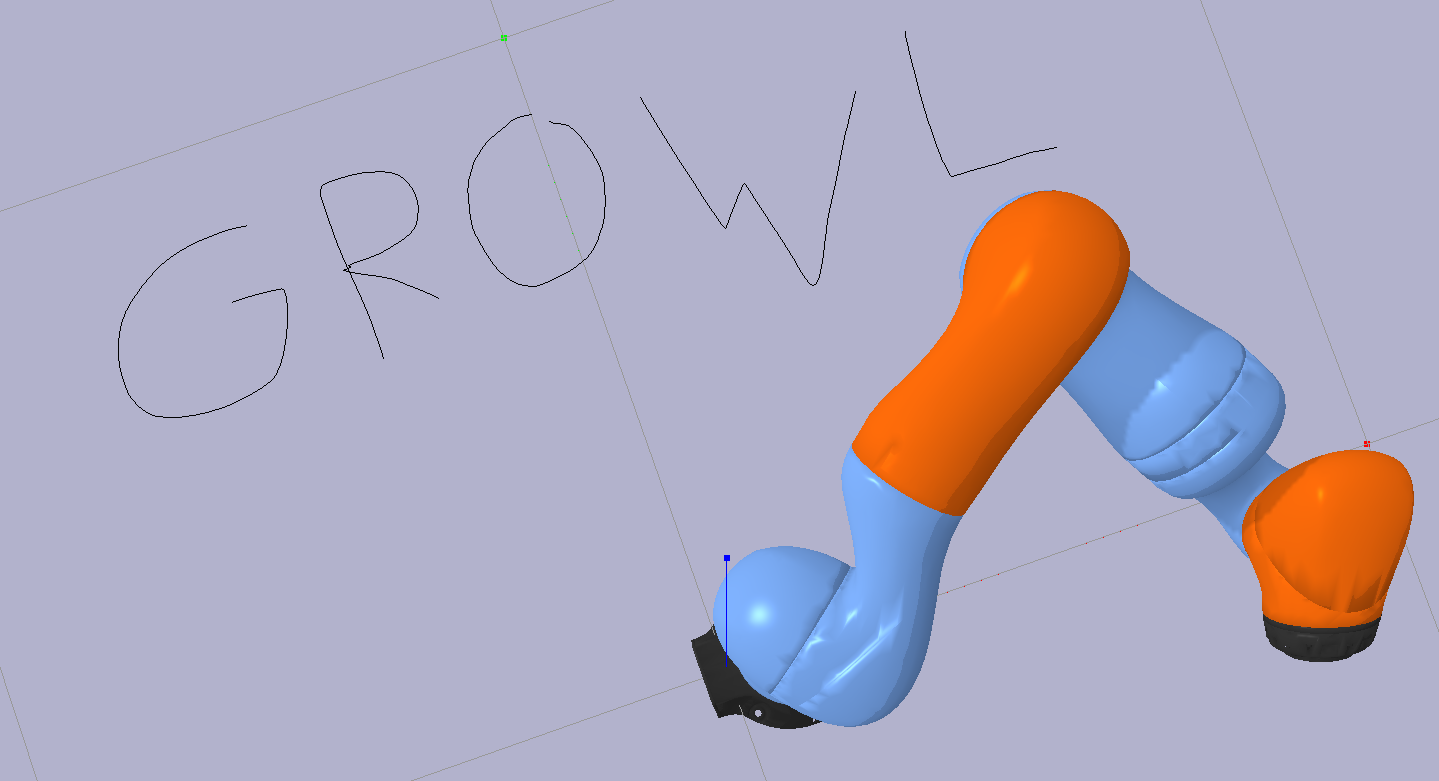
\includegraphics[scale=0.6]{images/2.png}\\
\end{center}

\section{LIMITATIONS}

This code runs well for the set of letters described in the previous sections - any letter that can be written in a single stroke and at every point has only one direction to move in. However, the script does have some limitations
\begin{enumerate}
    \item As described above, the script fails to track trajectories corresponding to certain complex alphabets such as K, X, etc. This is because the imitation learning algorithm used, i.e., {\it Random Forest} was unable to predict the velocities at certain input positions where multiple strokes cross over. This maybe solved using a much better learning algorithm tailor-made for such a use-case or to break multi stroke letters into different stroke based instances which can then be used while training the model
    \item The code does not {\it write} letters dynamically. There are separate blocks of code that write different alphabets; in order to write another letter or change the letter, the whole block needs to be modified. One way to solve this would be create a single nested list and keep appending the different velocities corresponding to the different letters {\it (along with the required gaps)} and then uses that as an input to the robot
    \item The simulation does not employ any form of manual disturbance rejection. If the arm is suddenly moved to a new position forcibly, the end effector will keep writing instead of pausing till the original state is restored. This can be solved by employing an intelligent logic that turns {\it user debug line} off whenever a disturbance is detected
\end{enumerate}

\bigskip

\section{REFERENCES}
\begin{enumerate}
    \item Data from { \it Pignat, E. and Calinon, S. (2017). Learning adaptive dressing assistance from human demonstration. Robotics and Autonomous Systems 93, 61-75.}
    \item Actual Dataset from {\it https://gitlab.idiap.ch/rli/pbdlib-python/-/tree/master/pbdlib/data/2Dletters}
    \item Scikit-learn library {\it https://scikit-learn.org/stable/index.html}
    \item Base code for PyBullet IK Sim: {\it https://github.com/McGIll-COMP-766-ECSE-683-Fall-2020/python-examples}
\end{enumerate}

%------------------------------------------------

\end{document}
